% ------------------------------------------------------------------------------|
% -----------------------------------------------------------------------------|
% ----------------------------------------------------------------------------|
\section{Funcionamiento}
% ----------------------------------------------------------------------------\
% -----------------------------------------------------------------------------\
% ------------------------------------------------------------------------------\

\subsection{Info Perros}

Este bot se le han cargado datos informativos sobre los perros, un ejemplo 
de ejecución es el siguiente con las líneas:

\begin{itemize}
    \item Hola
    \item ¿Cuánto ejercicio necesita mi cachorro?
    \item ¿Cuál es la mejor forma de entrenar a mi perro?    
\end{itemize}

\begin{center}
    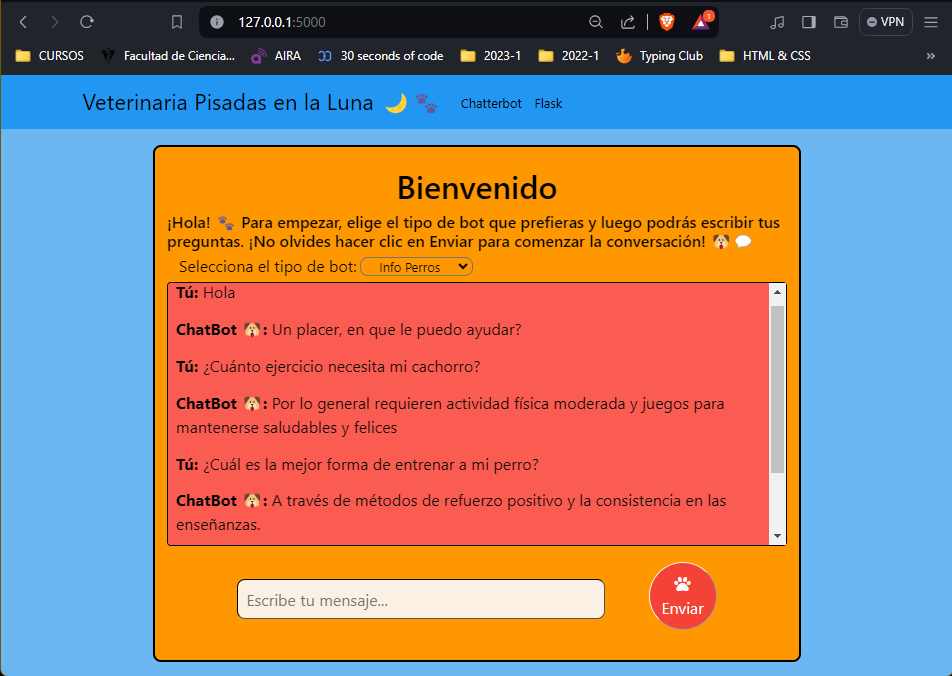
\includegraphics[scale = .5]{IMA/infoPerro.png}
\end{center}

\begin{center}
    Podemos notar que la pagina tiene un menú seleccionable.\\

    Dependiendo de con que bot queramos conversar, será el que seleccionemos.\\

    Al cambiar de bot se va a reiniciar el char    
\end{center}

\begin{center}
    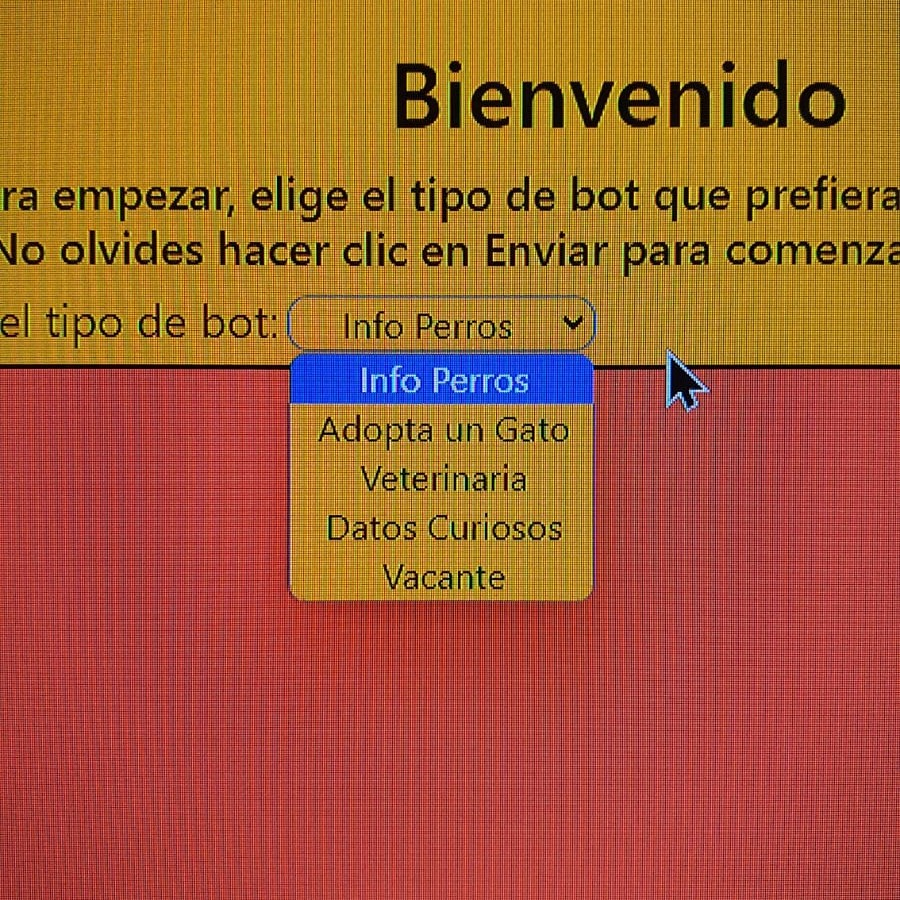
\includegraphics[scale = .2]{IMA/optiones.jpg}
\end{center}

\subsection{Adopta un gato}

Este bot se le han cargado datos para que un usuario por medio del color 
de gato que escoja pueda adoptar un gato y conocer sobre su nueva mascota. Un ejemplo 
de ejecución es el siguiente con las líneas:

\begin{itemize}
    \item Quiero adoptar un gato
    \item Un gato color blanco
    \item Que le doy de comer a mi gato?
\end{itemize}

\begin{center}
    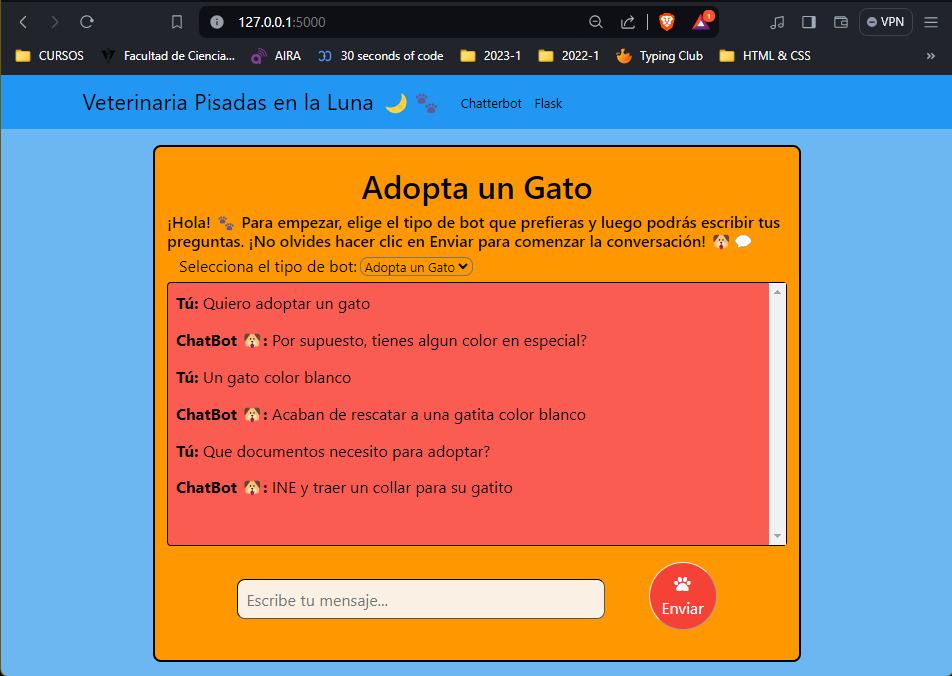
\includegraphics[scale = .5]{IMA/gato.png}
\end{center}

\subsection{Veterinaria}

Este bot se encarga de dar datos relevantes sobre la veterinaria. Un ejemplo de ejecución es el siguiente con las líneas:

\begin{itemize}
    \item ¿Que servicios ofrecen?
    \item ¿Cuáles son sus costos?
    \item ¿Costo de vacunas?
\end{itemize}

\begin{center}
    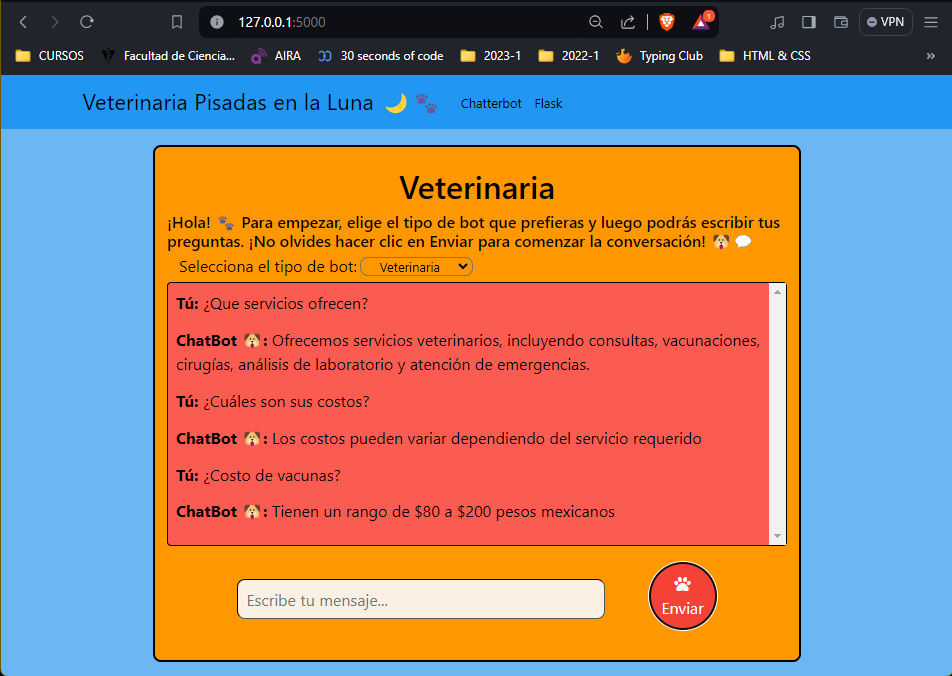
\includegraphics[scale = .5]{IMA/veterinaria.png}
\end{center}


\subsection{Datos Curiosos}

Con este bot te llenaras de información 
sobre curiosidades de animales al rededor 
del mundo. Un ejemplo de ejecución es 
el siguiente con las líneas y basta con 
poner el nombre del animal

\begin{itemize}    
    \item Oso polar
    \item Delfín
    \item Canguro
\end{itemize}

\begin{center}
    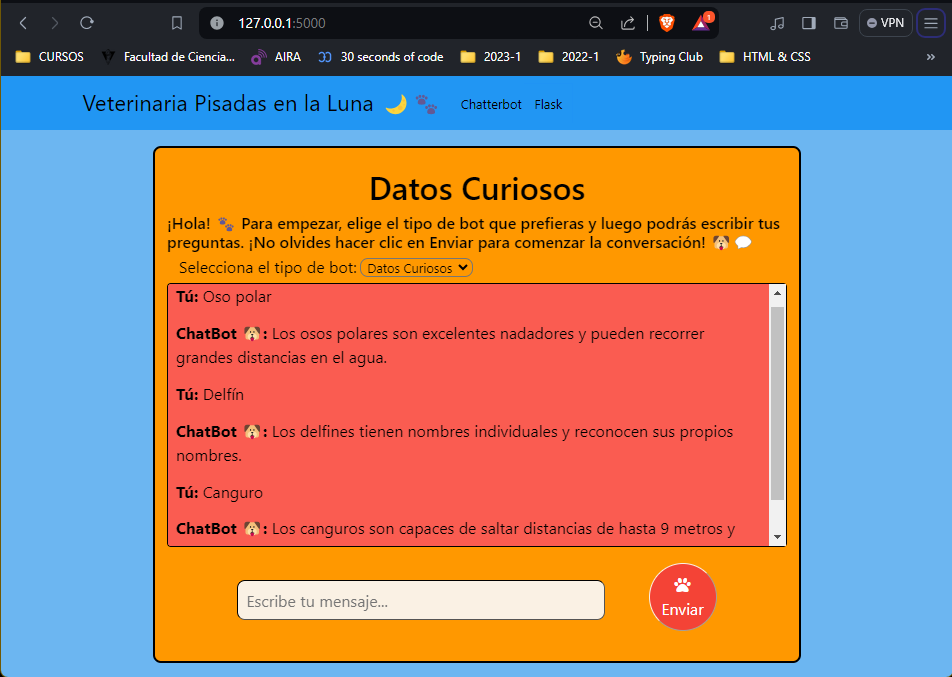
\includegraphics[scale = .5]{IMA/curiosos.png}
\end{center}


\subsection{Vacante}

Ahora simularemos una entrevista para entrenar
al equipo de trabajo de la veterinaria, para 
comenzar escribir: \textit{Iniciar Entrevista} y para cada 
pregunta se debe numerar, seguido un guion medio y una de estas 
tres respuestas según sea el caso: \textit{bajo, medio o alto}. 
Un ejemplo de ejecución es el siguiente con las líneas:

\begin{itemize}    
    \item Iniciar Entrevista
    \item 1-medio
    \item 2-alto
\end{itemize}

\begin{center}
    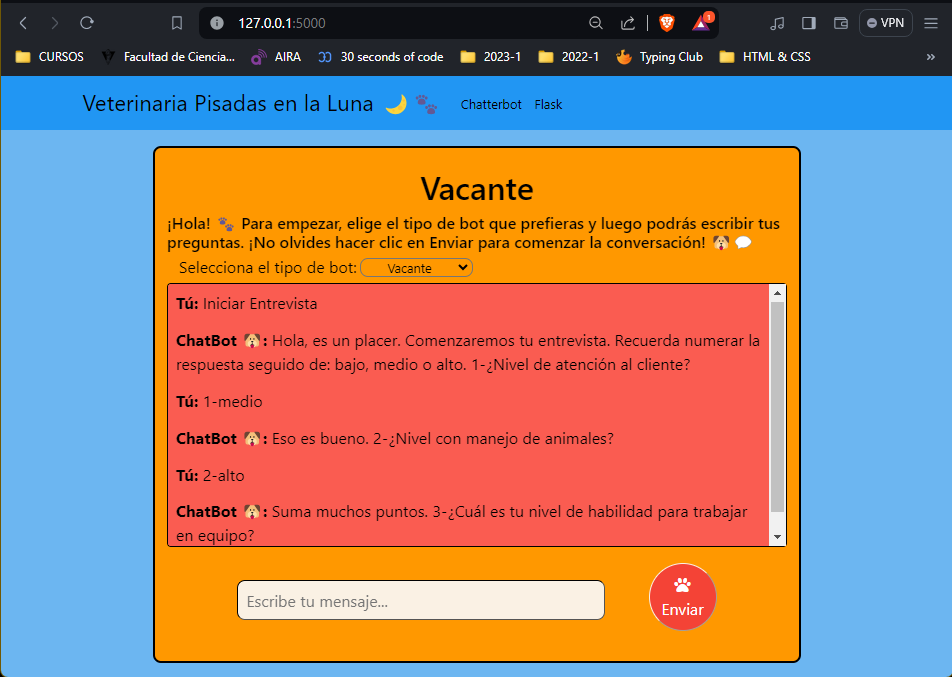
\includegraphics[scale = .5]{IMA/vacante.png}
\end{center}